\documentclass[tikz]{standalone}
\standaloneconfig{border=0.3cm}
\usepackage{tikz}
\usetikzlibrary{shapes, automata, arrows, positioning, fit, backgrounds, shapes.geometric, matrix}
\tikzstyle{block} = [rectangle, draw,
    text width=9em, text centered, rounded corners, minimum height=3.5em]
\tikzstyle{bordertext} = [text centered, rotate=270]
\tikzstyle{line} = [draw, -latex']

\begin{document}

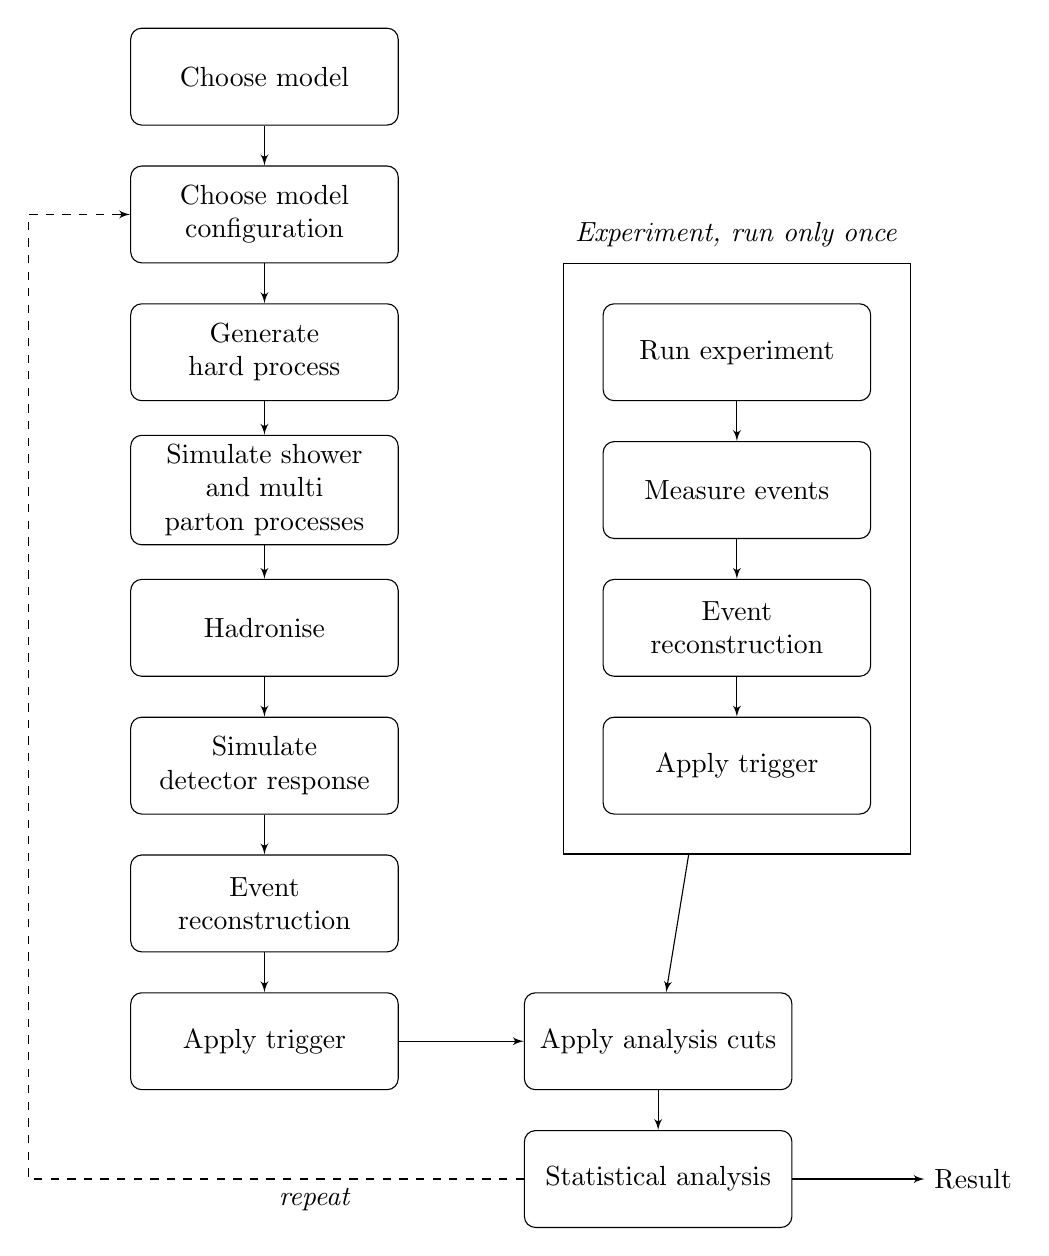
\begin{tikzpicture}[node distance = 1.75cm, auto]
  % Place nodes
  % Simulation
  \node[block] (model)    {Choose model};
  \node[block, below of=model] (config)   {Choose model configuration};
  \node[block, below of=config] (hard)     {Generate hard process};
  \node[block, below of=hard] (radiate)  {Simulate shower and multi\\ parton processes};
  \node[block, below of=radiate] (hadron)   {Hadronise};
  \node[block, below of=hadron] (detector) {Simulate\\ detector response};
  \node[block, below of=detector] (recon) {Event\\ reconstruction};
  \node[block, below of=recon] (trigger) {Apply trigger};
  % Experiment
  \node[block, right of=hard, node distance=6cm] (exp) {Run experiment};
  \node[block, right of=radiate, node distance=6cm] (measure) {Measure events};
  \node[block, right of=hadron, node distance=6cm] (recon2) {Event\\ reconstruction};
  \node[block, right of=detector, node distance=6cm] (trigger2) {Apply trigger};
  \begin{scope}[on background layer]
  \node[draw, fit=(exp) (trigger2), inner sep=5mm] (expblock){};
  \end{scope}
  \node (text) at (6.0, -2.0) {\textit{Experiment, run only once}};
  % Statistics
  \node[block, right of=trigger, node distance=5cm] (selection) {Apply analysis cuts};
  \node[block, below of=selection] (stat) {Statistical analysis};
  \node[right of=stat, node distance=4cm] (result) {Result};

  % Draw edges
  \path [line] (model) -- (config);
  \path [line] (config) -- (hard);
  \path [line] (hard) -- (radiate);
  \path [line] (radiate) -- (hadron);
  \path [line] (hadron) -- (detector);
  \path [line] (detector) -- (recon);
  \path [line] (recon) -- (trigger);
  \path [line] (trigger) -- (selection);

  \path [line] (exp) -- (measure);
  \path [line] (measure) -- (recon2);
  \path [line] (recon2) -- (trigger2);
  \path [line] (expblock) -- (selection);


  \coordinate[left of=stat, node distance=7cm] (inv1);
  \coordinate[left of=config, node distance=3cm] (inv2);

  \path [line] (selection) -- (stat);
  \path [line] (stat) -- (result);
  \path [line, dashed] (stat) -| node [near start] {\textit{repeat}} (inv1) -| (inv2)-- (config);
\end{tikzpicture}

\end{document}
